O \textit{benchmark} bench4Q define uma carga de trabalho, incluindo banco de dados, transações, regras de execução e de taxa de transferência e métricas de resposta.  Para expor a dinâmica de um sistema é necessário estimulá-lo através da carga de trabalho. Este componente é responsável por estimular o sistema através de cenários ou fenômenos de \textit{burstiness}. Essa implementação é composta por classes e métodos, esse conjunto de código é um componente básico do \textit{benchmark} que refere-se a uma unidade de trabalho genérico que envia a carga para o sistema. O \textit{burstiness} incluem solicitações HTTP, chamadas de procedimento remoto, invocações de serviços Web, transações de banco de dados, comandos interativos ou também mesmo poderia ser composto de múltiplas tarefas de processamento, por exemplo sessões de cliente que compreendem várias solicitações ao sistema, etc \cite{Kounev2005}. Segundo \citeonline{Nobile2013} uma alteração na entrada (carga de trabalho) fará com que o sistema saia do estado de regime estacionário e entre em um período de regime transiente que descreve a dinâmica de um sistema, o regime transiente é calculado para uma entrada degrau unitário.

O objetivo deste trabalho é estender a carga de trabalho do \textit{benchmark} Bench4Q de tal maneira que permite-se estimular o sistemas a apresentar a sua dinâmica, assim possibilitando a analise transiente do sistema. 

Conforme apresentado no Capitulo \ref{chapter:revisao}, o \textit{benchmark} Bench4Q oferece uma interface gráfica para configuração e colete dos dados, o que facilita a sua operação e analise. A proposta da extensão deste trabalho é manter o padrão de usabilidade e possibilitar a modulação da carga de trabalho. Sendo assim, também, via interface gráfica, com o preenchimento de um conjunto de parâmetros será possível a geração modulada da carga, com os descritos a seguir:
\begin{itemize}
	\item \textbf{Tempo de planejamento de carga:} Um período de tempo em que a carga de trabalho é modulada, caracterizado a mudança do comportamento das requisições de maneira programada;
	\item \textbf{Tipo de modulação:} conforme apresentado no \ref{chapter:revisao}, a modulação será apresenta conforme as funções ou sinais proposto por \citeonline{Hellerstein2004};
	\item \textbf{Tempo de interrupções:} Período de interrupções/pausa após o \textit{Tempo de planejamento de carga},
	\item \textbf{Quantidade de clientes na modulação:} reservar uma quantidade de clientes (EBs, para o caso do Bench4Q) que estão com dedicação exclusiva para a modulação da carga
\end{itemize}

Através da nova interface, que recebe os parâmetros para a modulação da carga, espera-se a modular cargas conforme os exemplos apresentados na figura	\ref{fig:cargas-moduladas-exemplos}, esses exemplos são derivados das funções apresentadas por \citeonline{Hellerstein2004}. Com esse tipo de variação da carga no decorrer do tempo é possível estimular o sistema de maneira a admirar a sua dinâmica.  Para \citeonline{Feitelson2015} o objetivo é, de ser capaz de criar cargas de trabalho que pode ser utilizado em estudos de avaliação de desempenho. 
A carga de trabalho \ref{fig:degrau-positivo}, talvez seja a de maior interesse e impacto para o trabalho de \citeonline{Edwin2015}. Pois a carga se inicia piano e moderada, porém terá um crescimento repentino e brusco podendo se manter perene, porem terá uma queda voltando ao patamar inicial. Já carga representada pela figura \ref{fig:degrau-negativo}, tem comportamento oposto a \ref{fig:degrau-positivo}, inicialmente a carga esta é seu mais alto nível e com potência máxima, porém tem uma queda brusca e repentina levando a carga a um baixo nível se mantendo por um período e da mesma maneira que caiu, subirá nas mesmas inversas proporções, mantendo-se até o final. Por fim, a carga modulada conforme a figura \ref{fig:onda-gradrada}, oscila da uma baixa intensidade á máxima intensidade. sempre com alterações a brusca e repentina e com os mesmos intervalos de unidade de tempo.
 
\begin{figure}[!htb]
	\centering
	\begin{subfigure}[b]{0.45\textwidth}
		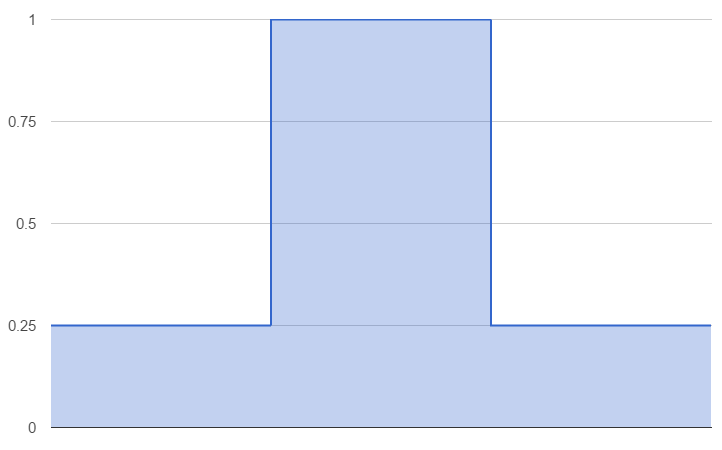
\includegraphics[width=\textwidth]{carga-sintetica1.png}
		\caption{Degrau positivo}
		\label{fig:degrau-positivo}
	\end{subfigure}
	~
	\begin{subfigure}[b]{0.45\textwidth}
		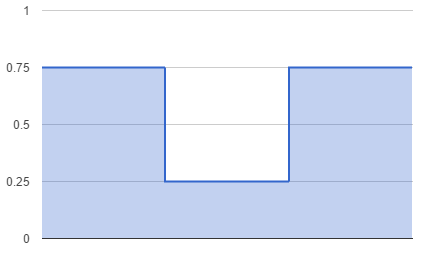
\includegraphics[width=\textwidth]{carga-sintetica2.png}
		\caption{Degrau negativo}
		\label{fig:degrau-negativo}
	\end{subfigure}
	~
	\begin{subfigure}[b]{0.45\textwidth}
		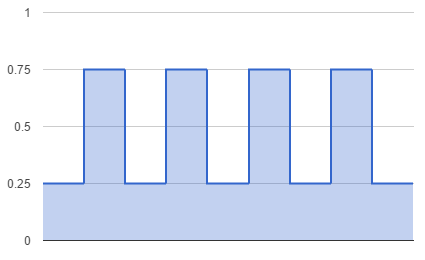
\includegraphics[width=\textwidth]{carga-sintetica3.png}
		\caption{Onda quadrada}
		\label{fig:onda-gradrada}
	\end{subfigure}
	\caption{Possibilidade de cargas moduláveis}
	\label{fig:cargas-moduladas-exemplos}
\end{figure}


Para \citeonline{Binnig2009} os serviços em nuvem de hoje diferem entre outros pelo custo, desempenho, garantias de consistência, balanceamento de carga, \textit{caching}, tolerância a falhas, SLA e linguagem de programação. O Bench4Q trata-se de um \textit{website} de um \textit{e-commerce}, segundo \citeonline{Dong2014} a maioria dos sites modernos usam uma arquitetura \textit{multi-tier}. Esta arquitetura particiona o processo de aplicação em múltiplas camadas. Cada camada fornece uma determinada funcionalidade. Uma vantagem de tal arquitetura é que pode proporcionar um elevado nível de escalabilidade e flexibilidade. No entanto, a alocação de recursos entre esses níveis será mais difícil devido à interdependência entre as camadas. Para a discussão deste trabalho, assumimos um sistema de \textit{n-tiers} que consiste nos seguintes componentes:

\begin{itemize}
	\item Gerador de Carga (\textit{Workload})
	\item Balanceador de carga (\textit{Load Balancer})
	\item Servidor Físico (\textit{Hypervisor})
	\item Servidor de dados (\textit{Data base})
\end{itemize}


\begin{figure}[!htb]
	\centering
	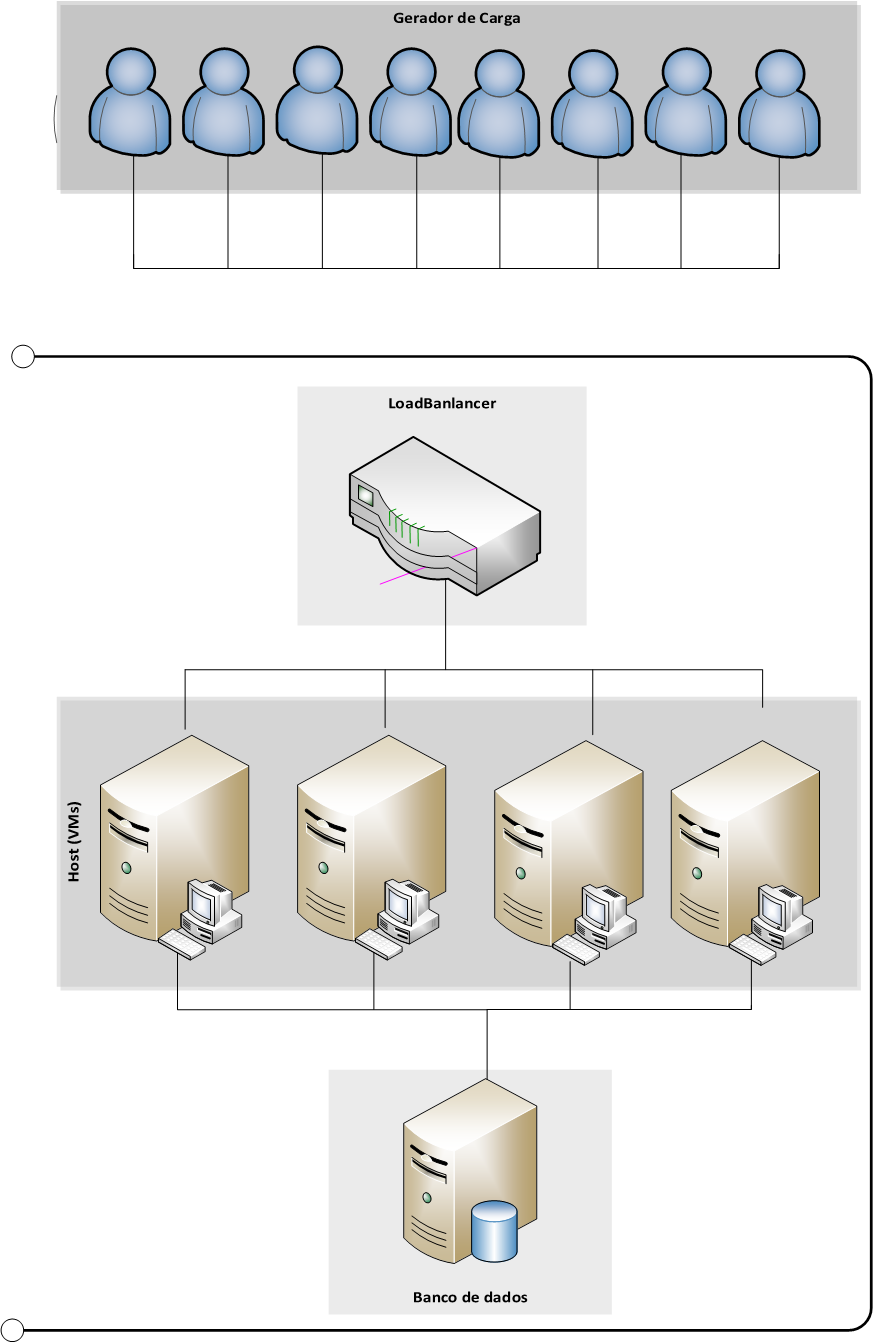
\includegraphics[scale=0.55]{arquitetura-experimento.png}
	\caption{Arquitetura do experimento}
	\label{fig:arquitetura-experimento}
	\fautor
\end{figure}

A arquitetura definida reflete no ambiente composto conforme a figura\ref{fig:arquitetura-experimento}. O ambiente utilizado para execução dos experimentos é apresentado na Tabela \ref{tab:configuracao_maquinas}.
Foram utilizadas oito unidades para a geração de carga de trabalho (\textit{workload}) que atuam como clientes dos serviços, uma unidade de balanceamento de carga e 4 servidores atuando como provedor de serviços e uma unidade executando o banco de dados a ser consultado pelo provedor de serviços.

\begin{table}[htb]
	\centering
	\caption{Especificação do ambiente de execução dos experimentos}
	\label{tab:configuracao_maquinas}
	\begin{tabularx}{\textwidth}{|r|c|X|} \hline\hline
		\textbf{Componente}    & \textbf{Quantidade} & \textbf{Configuração} \\ \hline
		\textit{Workload}      & 8 Unidades          & Intel Core 2 Quad Q6600 2.4GHz, 4GB de RAM \\
		\textit{Load Balancer} & 1 Unidade           & Intel Core 2 Quad Q6600 2.4GHz, 4GB de RAM \\
		\textit{Hosts}         & 4 Unidade           & Intel Core 2 Quad Q6600 2.4GHz, 4GB de RAM \\
		\textit{Data base}     & 1 Unidade           & AMD FX-8320 Vishera Eight-Core 3.5GHz, 24GB de RAM \\
		\hline
	\end{tabularx}
	\fdadospesquisa
\end{table}

De acordo com \citeonline{KaiSachs2010}, uma metodologia de desenvolvimento de \textit{benchmarks} deve incluir em seu processo de desenvolvimento, bem como a sua execução e a análise dos seus resultados. Para tanto é necessário medir o comportamento do sistema com a base me métricas. A métrica é uma função que transforma resultados medidos em uma forma facilmente compreendida \cite{Folkerts2013}. As métricas de referência deve permitir caracterizar e quantificar o comportamento do sistema quando enfrenta perturbações (ou seja, falhas, ataques, e variações de ambiente operacional) \cite{Marco2012}. As métricas tradicionais, de analise estacionaria, não podem capturar os comportamentos transitórios do sistema em resposta a modulação da carga de trabalho.

No contexto de avaliação transiente, \citeonline{Rosu1997} afirma que a reatividade da métrica é muitas vezes mais importante do que a otimização da mesma, no mesmo trabalho, \citeonline{Rosu1997} apresenta a característica e comportamento de uma métrica transiente, conforme ilustrado pela figura \ref{fig:transient-metric}, que são: 
\begin{itemize}
	\item \textbf{\textit{Reaction Time} (Tempo de reação)} - o período entre a ocorrência da variação crítica e a conclusão da promulgação realocação de correção;
	
	\item \textbf{\textit{Recovery Time} (Tempo de Recuperação)}  - o intervalo entre a conclusão promulgação e da restauração de um nível de desempenho aceitável;
	
	\item \textbf{\textit{Performance Laxity} (Frouxidão performance)} - a diferença entre o required v performance, e o desempenho em estado estacionário, após a redistribuição;
\end{itemize}


\begin{figure}[!htb]
	\centering
	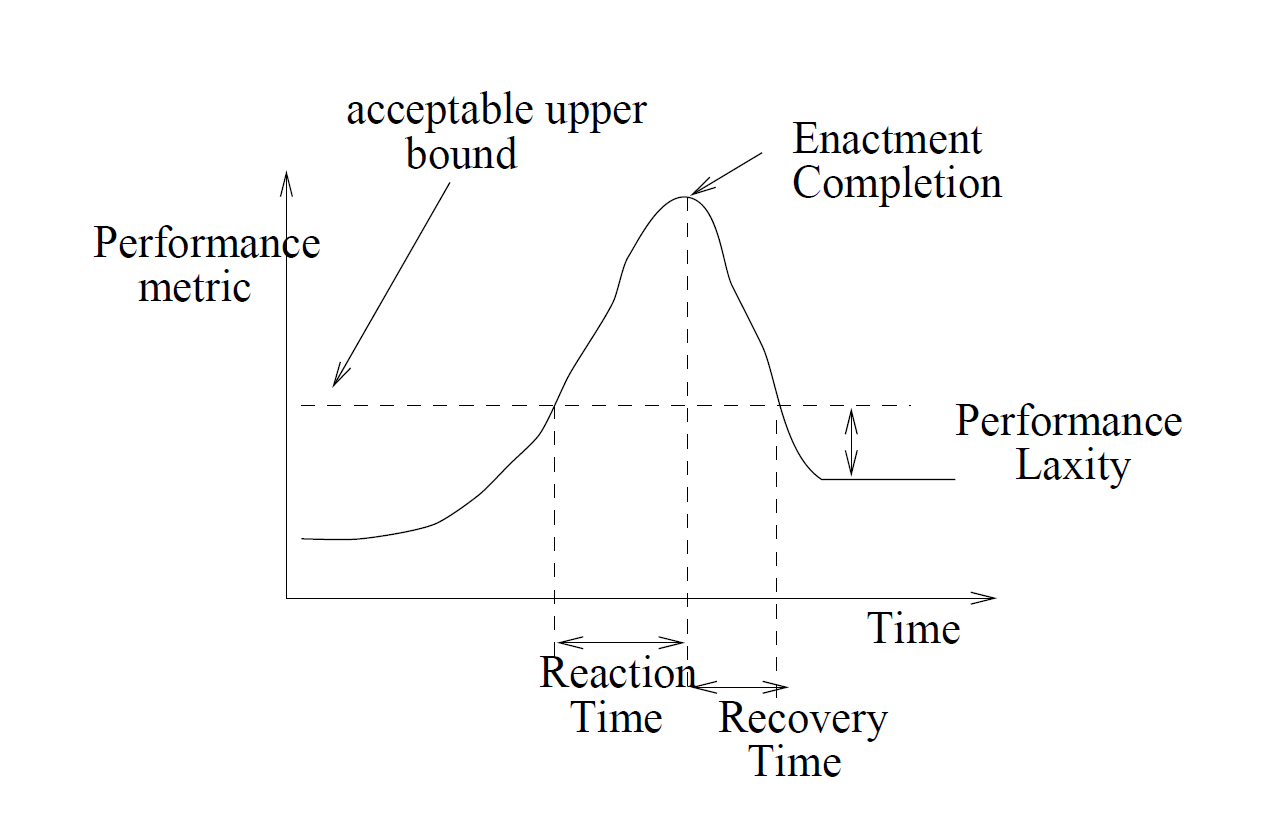
\includegraphics[scale=0.4]{transient-metric.png}
	\caption{Comportamento de métrica transiente}
	\label{fig:transient-metric}
	\fdireta{Rosu1997}		
\end{figure}


A métrica em questão deve ser identifica dentro da realidade e necessidade em que se encontra o sistemas a ser avaliado. Logo será de uma ingenuidade fixar um conjunto de métricas para um sistema desconhecido, o importante é que ela tenha o comportamento e as características apresentadas. Existem diversos trabalhos dedicados que identificam métricas transiente em vários contextos como o \citeonline{Binnig2009}, \citeonline{Lu2000} e \citeonline{Rosu1997}.
\citeonline{Binnig2009} afirma que os \textit{benchmarks} tradicionais são principalmente preocupados com o desempenho e o custo de sistemas estáticos e essas métricas ainda tem relevância para as aplicações em nuvem, mas é necessário medir diferentes métricas para sistemas escaláveis (ou seja, dinâmico) onde os recursos vêm e vão. Ainda \citeonline{Binnig2009} enfatiza que os novos \textit{benchmarks} devem relatar métricas diferentes do que os benchmarks existentes: 
\begin{citacao}
	Em vez de medir o desempenho médio de um sistema estático em carga máxima, as novas métricas devem refletir a capacidade dos serviços em nuvem para se adaptar a uma mudança de carga com relação ao desempenho e custos. Além disso, uma métrica adicional também deve cobrir a robustez desses serviços contra falhas de nós individuais.
\end{citacao}

As métricas definidas precisam refletir o cenário de dinâmica do sistema, logo é interessante cobrir cada um dos níveis da arquitetura proposta:
\begin{itemize}
	\item \textbf{Conexões por segundo (Load Balancer):} Conforme sugerido por \citeonline{Binnig2009}, medir a escalabilidade através do aumento dos interações web emitidos por segundo ao longo do tempo e de forma contínua contando o interação web que são respondidas em um intervalo de tempo de resposta,
	\item \textbf{Tempo de resposta (\textit{browsers}):} \citeonline{helder2014}, em um sistema dinâmico, cuja transformação entrada-saída não ocorre em tempo zero, mas é sujeita a uma inércia advinda dos processos físicos associados, possuem uma inércia intrínseca que atrasa o efeito que uma entrada terá na saída, esses efeitos refletem na consequência comportamentos diversos que incluem retardo no tempo de resposta e possíveis oscilações e definem a estabilidade do sistema, 
	\item \textbf{Taxa de utilização da CPU (VMs):} \citeonline{Nobile2013} afirma que diversas métricas podem ser analisadas para verificar o desempenho das máquinas virtuais, e cita alguns exemplos, como o tempo de inicialização, a taxa de utilização de CPU, o tempo médio de resposta e o \textit{throughput}, e usualmente, as máquinas virtuais hospedam serviços de interesse ao cliente que e respondem a uma carga de trabalho imposta por usuários através de requisições.
	\item \textbf{Taxa de utilização da CPU e taxa de transferência de I/O:} O trabalho apresentado por \citeonline{wang2009}, que lida com uma carga de trabalho variante no tempo e de intensiva demonstrando que CPU e I/O podem ser utilizadas para prever as necessidades dos recursos de um banco de dados e para orientar a alocação de recursos \textit{on-demand} de acordo com a exigência de carga de trabalho.
\end{itemize}
%• custo de capital: O custo de hardware e software adicional necessário para um sistema de HA em comparação com um sistema não-HA outra forma equivalente.
%• impacto Performance: O impacto para o desempenho de recursos de alta disponibilidade durante as operações normais em comparação com o sistema de não-HA.
%• Tempo de recuperação: O tempo para restaurar o serviço de banco de dados após a ocorrência de uma falha.


Os experimentos conduzidos neste trabalho consideraram três diferentes fatores de dois níveis cada, conforme aprestando na Tabela \ref{tab:fatores_niveis}. 

\begin{table}[htb]
	\centering
	\caption{Fatores e níveis dos experimentos}
	\label{tab:fatores_niveis}
	\begin{tabularx}{\textwidth}{|r|c|c|X|} \hline\hline
		\textbf{Fator}		& \textbf{\textit{Workload}} & \textbf{Banco de dados}  & \textbf{Politica de alocação de recursos} \\ \hline
		\textit{Nível 1}	&							 & Postgres					& Estática									\\
		\textit{Nível 2}	&							 & DB2						& Dinâmica									\\		
		\hline
	\end{tabularx}
	\fdadospesquisa
\end{table}


O primeiro fator refere-se à quantidade de clientes simultâneos requisitando o serviço Web, esses clientes são modulados conforme a configuração feita, sendo assim essa carga de trabalha estimulará o sistema a apresentar a sua dinâmica. O segundo fator associado a possibilidade de serem considerados diferentes tipos de serviço, assim este fator terá dois níveis de bancos de dados o Postgres e o DB2, o Bench4Q oferece o \textit{script} de criação de bando para ambos. O último e o terceiro fator, se refere a política de alocação de recursos, neste caso são dois níveis \textit{estática} (onde os servidores \textit{host} estão desde o princípio em execução e disponíveis.) e \textit{dinâmica} (onde os servidores são colocados à disposição conforme a oscilação da carga de trabalho), apesar deste tema não ter sido abordado neste trabalho, a utilização desse fator está relacionada a analise em todos os níveis da solução.

O planejamento de experimento e utilizado neste trabalho como avaliação de desempenho segue a abordagem do planejamento fatorial completo, em um total de 9 combinações. Logo, possibilita que todas as combinações possíveis dos fatores sejam examinados. Para cada experimento serão 5 repetições, totalizando 45 execuções dos experimentos, que utilizadas para determinar a média, o desvio padrão e o intervalo de confiança de 95\% .

Durante a execução dos experimentos pequenas aplicações, monitores, em cada um dos níveis da arquitetura são responsáveis por coletar algumas informações de interesse disponíveis, como a taxa de utilização de CPU e a quantidade de requisições simultâneas. Os valores produzidos pela experimentação foram adicionados em arquivos Excel (\textit{.xls}), esses dados foram processados pelo R \footnote{\url{https://www.r-project.org/}}.
